\subsection{Les pré-actionneurs}
Les \textbf{pré-actionneurs} remplissent la fonction \textit{distribuer} de la chaîne d'énergie. Ce sont eux qui  adaptent l'énergie puis la distribuent aux différents actionneurs. Ils \textbf{sont commandés par l'automate en vue de faire fonctionner les actionneurs}.

\UPSTIaRetenir{Un automate programmable \textbf{commande les pré-actionneurs} pour faire fonctionner les \textit{actionneurs}.}

\UPSTIexemple{%
\begin{minipage}[b]{.49\textwidth}
\centering
	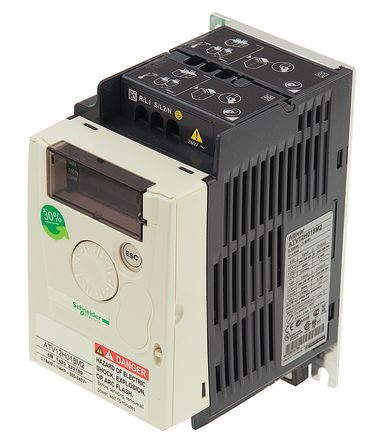
\includegraphics[width=.3\textwidth,height=.4\textheight,keepaspectratio]{images/varia_vitesse_mot_elec}

	Un variateur de vitesse pour moteur électrique adapte la tension d'alimentation du moteur pour en régler la vitesse.
\end{minipage}\hfill
\begin{minipage}[b]{.49\textwidth}
\centering
	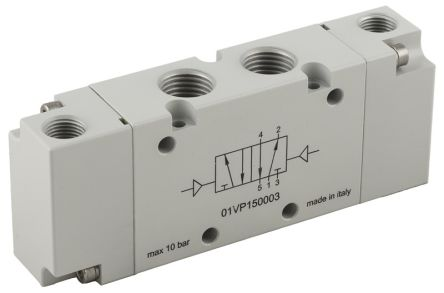
\includegraphics[width=.3\textwidth,height=.4\textheight,keepaspectratio]{images/distri_electroPneu}

	Un distributeur électro-pneumatique contrôle l'arrivée d'air comprimé dans les organes pneumatiques (vérin par exemple).
\end{minipage}
 %
}
